\documentclass{article}
\usepackage{fancyhdr}
\usepackage{tabularx}
\usepackage{geometry}
\usepackage{lipsum}
\usepackage{amssymb}
\usepackage{venndiagram}
\usepackage{subcaption}
\usepackage{wrapfig}
\usepackage{multicol}
\usepackage{float}
\usepackage{amsthm}
\usepackage{pdfpages}


\usepackage{caption}





% Seitenränder einstellen
\geometry{a4paper, left=2.5cm, right=2.5cm, top=2.5cm, bottom=2.5cm}

% Header definieren
\pagestyle{fancy}
\fancyhf{}
\renewcommand{\headrulewidth}{1pt}
\lhead{Anton Jagow, Lukas Dzielski}
\rhead{Ruprecht-Karls-Universität Heidelberg \\ MaFIn \\ Max-Emanuel Hlawatsch}
\lfoot{}
\rfoot{\thepage}

\begin{document}

\section*{Übungszettel \#4} % Setze die Nummer des Zettels

\begin{center}
    \begin{tabular}{|c|c|}
        \hline
        Aufgabe & Punkte \\
        \hline
        1 & \\
        2 & \\
        3 & \\
        \hline
        Gesamt & \\
        \hline
    \end{tabular}
\end{center}

\subsection*{Aufgabe 1}
\subsubsection*{(c = 6)}
\begin{center}
    \begin{tabular}{c|ccccccc}
        + & 0 & 1 & 2 & 3 & 4 & 5 & 6 \\
        \hline
        0 & 0 & 1 & 2 & 3 & 4 & 5 & 0 \\
        1 & 1 & 2 & 3 & 4 & 5 & 0 & 1 \\
        2 & 2 & 3 & 4 & 5 & 0 & 1 & 2 \\
        3 & 3 & 4 & 5 & 0 & 1 & 2 & 3 \\
        4 & 4 & 5 & 0 & 1 & 2 & 3 & 4 \\
        5 & 5 & 0 & 1 & 2 & 3 & 4 & 5 \\
        6 & 0 & 1 & 2 & 3 & 4 & 5 & 0 \\
    \end{tabular}    
\end{center} 
\begin{center}
    \begin{tabular}{c|ccccccc}
        * & 0 & 1 & 2 & 3 & 4 & 5 & 6 \\
        \hline
        0 & 0 & 0 & 0 & 0 & 0 & 0 & 0 \\
        1 & 0 & 1 & 2 & 3 & 4 & 5 & 0 \\
        2 & 0 & 2 & 4 & 0 & 2 & 4 & 0 \\
        3 & 0 & 3 & 0 & 3 & 0 & 3 & 0 \\
        4 & 0 & 4 & 2 & 0 & 4 & 2 & 0 \\
        5 & 0 & 5 & 4 & 3 & 2 & 1 & 0 \\
        6 & 0 & 0 & 0 & 0 & 0 & 0 & 0 \\
    \end{tabular}
\end{center}
\subsubsection*{(c = 7)}
\begin{center}
    \begin{tabular}{c|cccccccc}
        + & 0 & 1 & 2 & 3 & 4 & 5 & 6 & 7\\
        \hline
        0 & 0 & 1 & 2 & 3 & 4 & 5 & 6 & 7\\
        1 & 1 & 2 & 3 & 4 & 5 & 6 & 0 & 1\\
        2 & 2 & 3 & 4 & 5 & 6 & 0 & 1 & 2\\
        3 & 3 & 4 & 5 & 6 & 0 & 1 & 2 & 3\\
        4 & 4 & 5 & 6 & 0 & 1 & 2 & 3 & 4\\
        5 & 5 & 6 & 0 & 1 & 2 & 3 & 4 & 5\\
        6 & 6 & 0 & 1 & 2 & 3 & 4 & 5 & 6\\
        7 & 0 & 1 & 2 & 3 & 4 & 5 & 6 & 0\\
    \end{tabular}
\end{center}
    
\begin{center}
    \begin{tabular}{c|cccccccc}
        * & 0 & 1 & 2 & 3 & 4 & 5 & 6 & 7\\
        \hline
        0 & 0 & 0 & 0 & 0 & 0 & 0 & 0 & 0\\
        1 & 0 & 1 & 2 & 3 & 4 & 5 & 6 & 0\\
        2 & 0 & 2 & 4 & 6 & 1 & 3 & 5 & 0\\
        3 & 0 & 3 & 6 & 2 & 6 & 1 & 4 & 0\\
        4 & 0 & 4 & 1 & 5 & 2 & 6 & 3 & 0\\
        5 & 0 & 5 & 3 & 1 & 6 & 4 & 2 & 0\\
        6 & 0 & 6 & 5 & 4 & 3 & 2 & 1 & 0\\
        7 & 0 & 0 & 0 & 0 & 0 & 0 & 0 & 0\\
    \end{tabular}
        
\end{center}
\subsubsection*{(b)}
Man Strecht die erste Zeile und Spalte (die der 0). Man erkent aus den Tabellen das für d = 7 ansonsten keine 0 drinn vorkommt. Anders bei d = 6 das steht aber gegen der Definition des Zahlenbereichs weshalb das keine Verknüpfung auf dem Zahlenbereich ist.

\subsubsection*{(c)}
\begin{itemize}
    \item Die 1 ist das neutrale Element.
    \item Da \(a * a^{-1} = 1\) gilt und in jeder Zeile eine 1 existiert kann man daraus schließen das es zu jeder Zahl ein inverses gibt.
\end{itemize}

\subsection*{Aufgabe 2}
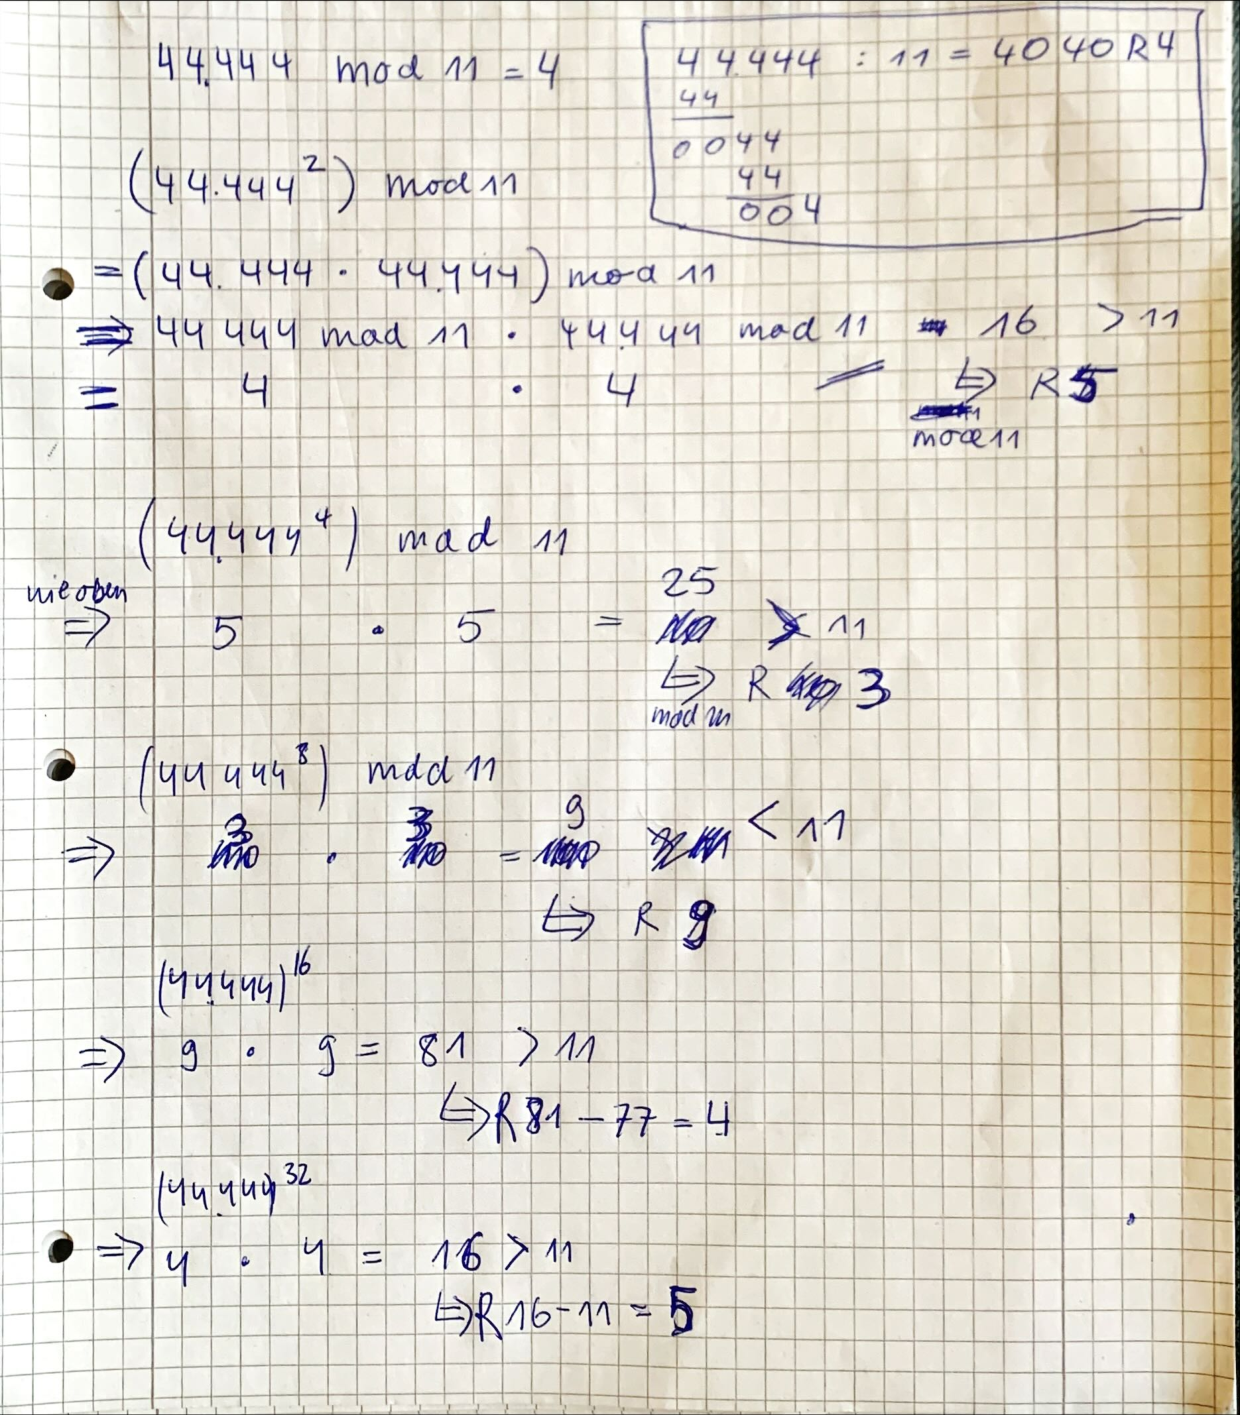
\includepdf[pages=-]{Aufgabe_2.pdf}
\end{document}
